\chapter{Sonorización del Proyecto}

Con el fin de cubrir todas las temáticas disponibles (Sección \ref{sec:tematicas}), hemos reunido una serie de plugins que nos permiten contar con un catálogo de timbres muy diversos. Todos los instrumentos utilizados son gratuitos. Adenás, hemos priorizado que sean plugins ligeros, de forma que la herramienta final no requiera de demasiado almacenamiento. No obstante, el usuario final de la herramienta puede cambiar facilmente dentro de Reaper los instrumentos cargados por otros plugins externos de su elección que haya instalado.

Además de generar sonidos, hay multitud de tareas que pueden realizar los plugins, como transformar el sonido o el MIDI, añadir reverberación, eco u otros efectos que veremos a continuación. Estos plugins se denominan plugins de efectos.

Reaper incluye algunos plugins de efectos de base, pero apenas tiene instrumentos virtuales, al contrario que otras DAWs populares que incluyen una buena cantidad de estos en su versión básica. Los efectos principales se nombran más adelante (Sección \ref{subsec:plugins-utilizados}).

\section{Presets}
Reaper nos permite guardar configuraciones de un plugin para usarlas más adelante, esto es lo que se conoce como \textit{preset}. La mayoría de plugins también permiten la opción de guardar presets dentro de su propia interfaz. Y de hecho, suelen traer algunos presets ya creados por el fabricante del plugin con sonidos o efectos que funcionan y que hemos aprovechado para nuestros presets.

\section{Plugins utilizados}\label{subsec:plugins-utilizados}
Vamos a detallar los timbres y los efectos más importantes presentes en las canciones generadas por la herramienta así como los plugins concretos que hemos usado para generarlos. 

En la Figura \ref{fig:Efectos-acompañamiento} podemos ver la cadena de efectos que utilizamos para una pista de acompañamiento (Sección \ref{subsec:instrumentos-principales}). Es similar a la cadena de efectos que usamos en otras pistas, añadiendo o quitando algún plugin dependiendo de las necesidades que hay que cumplir

\begin{figure}[h]
    \centering
    \includegraphics[width = 0.5\textwidth]{Imagenes/Bitmap/EfectosPistaAcompañamiento.png}
    \caption{Plugins en la pista de acompañamiento}
    \label{fig:Efectos-acompañamiento}
\end{figure}

% TODO: referenciar esta imagen y usarla de ejemplo para todo.
\begin{figure}[h]
    \centering
    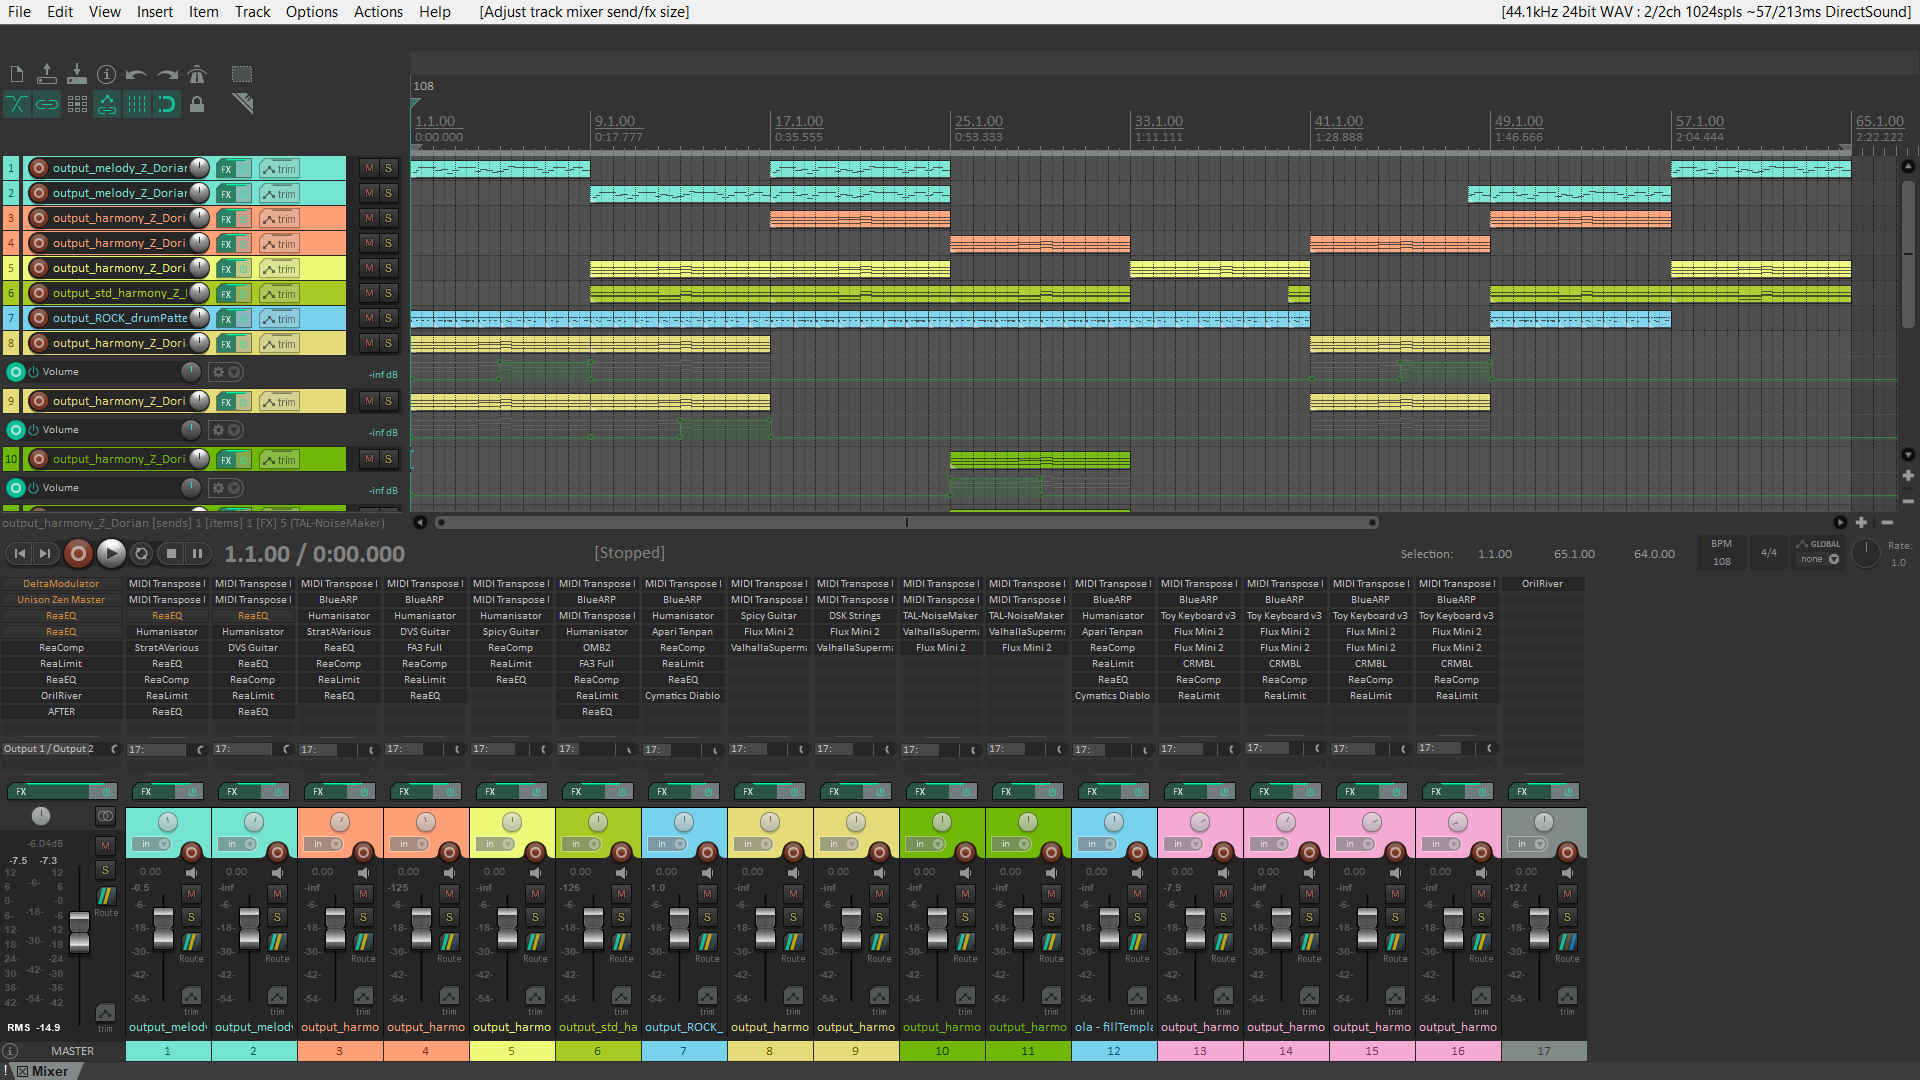
\includegraphics[width = 0.9\textwidth]{Imagenes/Bitmap/ArregloReaperMixer.png}
    \caption{Efectos utilizados en Reaper}
    \label{fig:ArregloReaperMixer}
\end{figure}

La lista completa de plugins que hemos utilizado puede encontrarse en el Apéndice \ref{Appendix:Key1}.

    \subsection{Instrumentos virtuales}\label{subsubsec:bluearp}
Hemos usado un gran número de plugins de instrumentos virtuales para lograr un amplio catálogo de timbres que cubren las distintas temáticas (Sección \ref{sec:tematicas}) y ofrecen variedad tímbrica para estas, ya que tenemos varios presets para cada pista (Sección \ref{sec:pistas}) y temática. Hemos priorizado la facilidad de instalación a la vez que la variedad, por eso usamos principalmente instrumentos sintetizados que simulan los timbres que buscamos.

En la Figura \ref{fig:Efectos-acompañamiento}, el instrumento virtual que hay cargado es el cuarto elemento (DPiano-A).

\subsection{Plugins auxiliares}\label{subsubsec:bluearp}
Utilizamos algunos plugins que nos proporciona Reaper para realizar algunas tareas:

\begin{itemize}
    \item \textbf{Transponer notas}: modificamos la señal MIDI recibida para subir o bajar semitonos dependiendo de la configuración recibida desde la app. En algunas pistas también usamos este plugin para subir o bajar una octava entera.

    \item \textbf{Comprimir y limitar}: cargamos dos plugins, ReaComp y ReaLimit, para intentar igualar el volumen lo máximo posible entre los distintos instrumentos.
    
    \item \textbf{Ecualizar}: cargamos un plugin ReaEQ para ecualizar el sonido. Junto con la compresión, logramos que el sonido de la pista se mezcle con el del resto de pistas de la mejor forma posible, dando a cada pista su espacio en el espectro de frecuencias.  
    
\end{itemize}



    \subsection{\textit{BlueArp}}\label{subsubsec:bluearp}
\textit{BlueArp} es uno de los plugins de efectos principales que utilizamos. Es un tipo de plugin que recibe una señal MIDI (Sección \ref{subsec:que-es-midi}) y la convierte en otra. Para que esto funcione debemos colocarlo antes en la cadena de efectos que los instrumentos virtuales, para transformar el MIDI antes de que sea convertido en sonido.

El principal uso de el plugin \textit{BlueArp} es hacer el trabajo de un arpegiador. Los arpegiadores reciben un acorde y lo transforman en un acorde arpegiado (Sección \ref{subsec:arpegios}). En nuestro caso, a parte de usarlo como arpegiador, lo usamos también para generar ritmos de acordes, líneas de bajo (Sección \ref{sec:lineas-de-bajo}), \textit{drum fills} (Sección \ref{subsubsec:generacion-drum-fills}), \textit{ear candy} (Sección \ref{sec:ear-candy})

En la Figura \ref{fig:BlueArp} podemos ver la interfaz del plugin \textit{BlueArp}. En la parte derecha de esta imagen podemos observar el patrón que transformará el MIDI entrante, un patrón de arpegio común. Este patrón tiene en cuenta la posición de las notas en un acorde comenzando por la nota más grave teniendo en cuenta que el acorde puede estar invertido (Sección \ref{subsec:inversiones})

En la Figura \ref{fig:CArpegiadoenMIDI} podemos ver primero un acorde de C en su forma básica. Esta será la señal MIDI que reciba el plugin arpegiador. A su derecha, la transformación que ha sufrido el MIDI tras pasar por BlueArp (con la configuración de la Figura \ref{fig:BlueArp}). 

\begin{figure}[h]
    \centering
    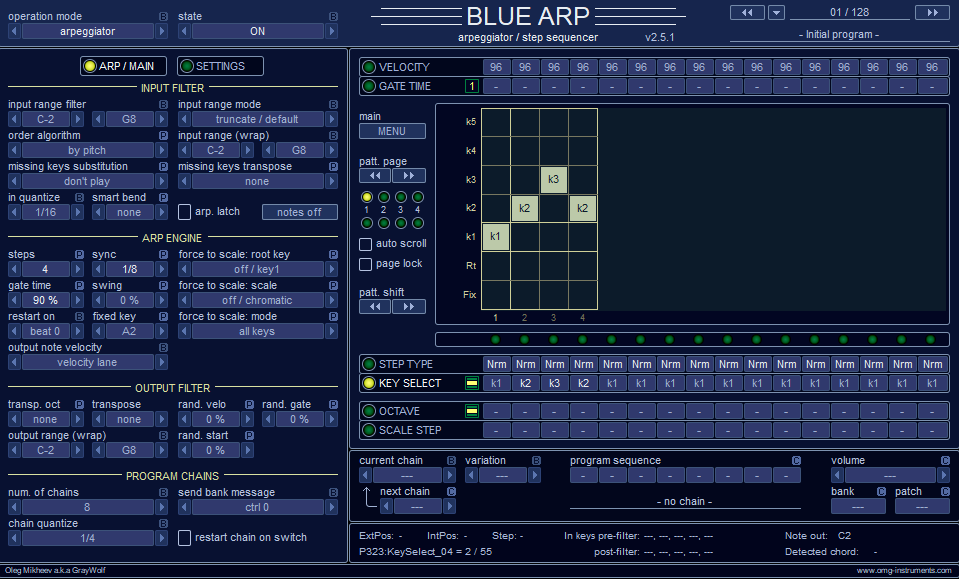
\includegraphics[width = 0.9\textwidth]{Imagenes/Bitmap/BlueArp.png}
    \caption{Interfaz de BlueArp haciendo un arpegio}
    \label{fig:BlueArp}
\end{figure}
    
\begin{figure}[h]
    \centering
    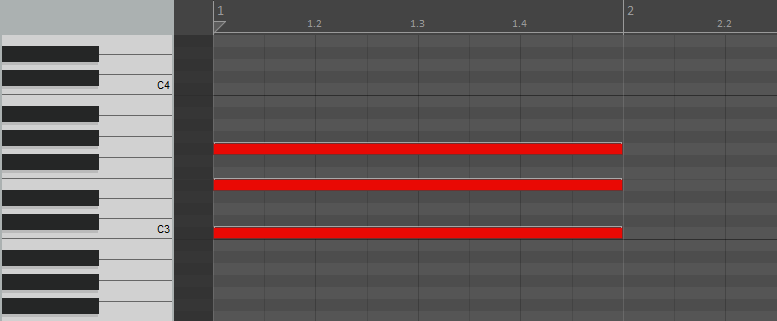
\includegraphics[width = 0.45\textwidth]{Imagenes/Bitmap/DoMayorMidi.png}
    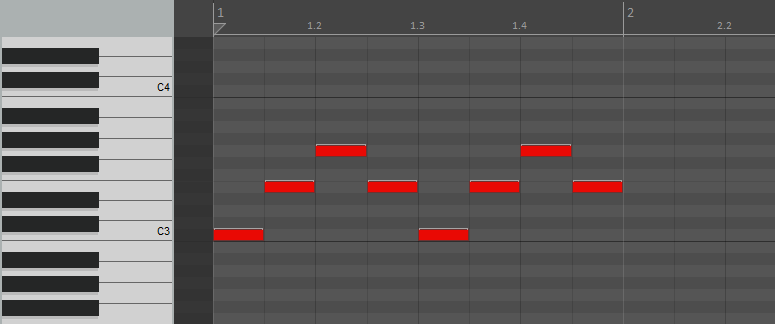
\includegraphics[width = 0.45\textwidth]{Imagenes/Bitmap/DoMayorMidiArpegiado.png}
    \caption{Acorde de C en MIDI arpegiado}
    \label{fig:CArpegiadoenMIDI}
\end{figure}

A parte de generar arpegios, de manera similar podemos usar \textit{BlueArp} para generar acordes enteros en una misma figura (en lugar de sólo una nota).

Lo mismo sucede cuando queremos hacer una línea de bajo (Sección \ref{sec:lineas-de-bajo}), 
cargamos un MIDI con acordes en la pista del bajo y usamos \textit{BlueArp} para que la señal MIDI resultante sólo tenga una nota cada vez, que será principalmente la nota fundamental del acorde.
    
    \subsection{Humanizador}\label{subsubsec:humanizador}
A la hora de producir una canción, si vas a crear los sonidos usando instrumentos virtuales en lugar de grabarlos, el productor puede encontrarse con que la música generada puede sonar robótica, sin vida. Esto se debe a que el MIDI es muy preciso en velocidad y tempo, hasta el punto de que no es realista el sonido que se obtiene, ya que ningún músico toca con la precisión perfecta de un ordenador.

Para solucionar este problema existe la humanización. En Reaper, podemos humanizar las notas en el propio rodillo de piano pulsando la tecla H. Como la idea es que nuestra herramienta requiera la menor intervención humana posible, podemos explorar otras alternativas para humanizar el MIDI.

Usaremos un plugin de efectos, que transformará el MIDI en otra señal MIDI, al igual que hacía \textit{BlueArp}. En concreto, hemos elegido el \textit{Humanisator} de \textit{Toby Bear}. Con este plugin transformamos una señal MIDI con una velocidad fija y a tempo exacto en una señal MIDI humanizada. Por ejemplo, en la Figura \ref{fig:CArpegiadoenMIDIHumanizado} convertimos el acorde que arpegiamos con BlueArp en la Figura \ref{fig:CArpegiadoenMIDI} en un acorde arpegiado humanizado (el color representa la velocidad de la nota), que ahora se parecería bastante a lo que un teclista grabaría con un controlador MIDI\footnote{\url{https://soundsmarket.com/blog/controlador-midi}}.


\begin{figure}[h]
    \centering
    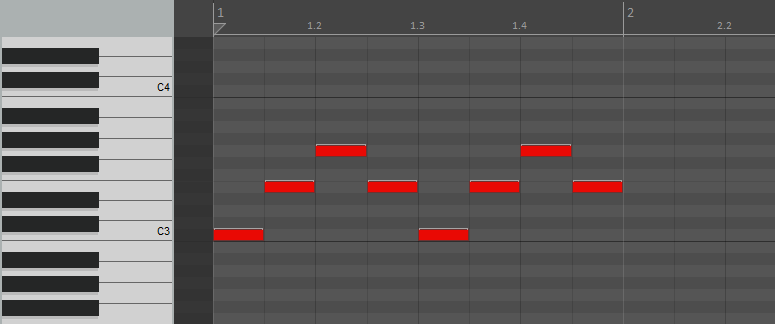
\includegraphics[width = 0.45\textwidth]{Imagenes/Bitmap/DoMayorMidiArpegiado.png}
    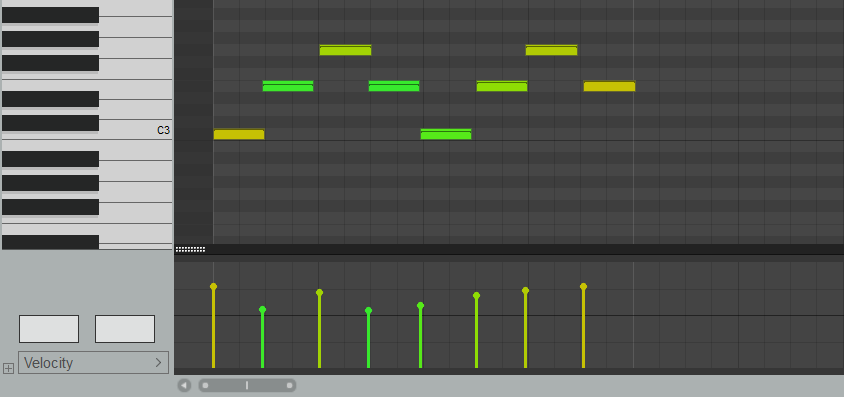
\includegraphics[width = 0.45\textwidth]{Imagenes/Bitmap/DoMayorMidiArpegiadoHumanizado.png}
    \caption{Acorde de C en MIDI arpegiado humanizado}
    \label{fig:CArpegiadoenMIDIHumanizado}
\end{figure}

    \subsection{\textit{Delay}}\label{subsubsec:delay}
El efecto de \textit{delay} genera un eco de un sonido recibido, repitiendo ese sonido de forma atenuada cierto tiempo después. 

Usamos este efecto para añadir algo más de presencia a los \textit{ear candy} (Sección \ref{sec:ear-candy}) en algunas ocasiones. Para lograr este efecto, usamos el plugin CRMBL de UnplugRed.

    \subsection{\textit{Reverb}}\label{subsubsec:reverb}
La reverberación es el efecto encargado de colocar un sonido en un entorno concreto, pues simula el rebote del sonido en distintas superficies. Sin nada de reverberación, es más dificil lograr que un sonido suene natural.

La reverberación puede añadirse a un sólo sonido o a una mezcla de sonidos, lo que hace que suenen mejor en conjunto, como si estuvieran situados en el mismo sitio.

La manera correcta de añadir reverb a una mezcla es realizar un envío\footnote{\url{https://dnamusic.edu.co/los-efectos-de-envio/}} desde todas las pistas a una nueva pista, en la cual cargaremos nuestro plugin de reverb con la señal \textit{dry} a menos infinito, es decir, en esta pista sólo sonará la reverb. De esta forma podemos controlar cuanta señal enviamos desde cada pista a la reverb. Esto es muy útil por ejemplo para enviar más señal de los instrumentos principales, o para enviar menos señal del bajo o la batería y así no ocupen más espacio del que les toca en la mezcla.

Esta forma de trabajar con la reverberación es muy cómoda y sencilla de montar para un usuario de Reaper. Pero no hemos conseguido montarla con ReaScript (Sección \ref{subsec:reascripy}) debido a sus limitaciones. Es por eso por lo que hemos añadido la reverberación a los efectos del máster, lo cuál no nos proporciona todo el control que nos gustaría sobre el sonido de la reverberación, pero cumple su función.

    \subsection{Mezcla}
El máster en reaper es una pista por la que pasan todos los sonidos del resto de pistas, es la pista con el sonido de la mezcla final. Por tanto, cuando cargamos un plugin en la pista de máster, afecta a todos los sonidos de la canción. Los plugins que cargamos en el máster de base se pueden ver en la Figura \ref{fig:Efectos-master}.
    
Como se explica en el apartado de la reverberación (Sección \ref{subsubsec:reverb}), cargaremos un plugin de reverberación en el máster que afectará a todas las demás pistas y aportará coherencia a la mezcla resultante. Usaremos para esto el plugin \textit{OrilRiver} de Denis Tihanov, aunque el usuario de la herramienta puede reemplazarlo por cualquier otro plugin de reverberación de su elección que tenga instalado.

A continuación usamos un compresor y un limitador para darle algo más de volumen y cohesión a la mezcla final, un ecualizador para tratar distintas frecuencias dependiendo de la temática de la canción, de nuevo una instancia del \textit{OrilRiver} para expandir el estéreo de la mezcla y por último un plugin \textit{AFTER} de TWestProductions, que se encarga de masterizar\footnote{\url{https://www.landr.com/es/que-es-la-masterizacion/}} de forma muy sencilla la canción.


\begin{figure}[h]
    \centering
    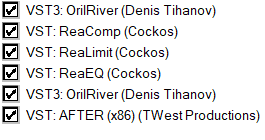
\includegraphics[width = 0.5\textwidth]{Imagenes/Bitmap/EfectosMaster.png}
    \caption{Plugins en el master}
    \label{fig:Efectos-master}
\end{figure}    

    \subsection{Efectos en la mezcla}\
Desde la ventana de la herramienta (Sección \ref{sec:TK:app}) podemos marcar algunos \textit{checkboxes} que añadirán varios plugins de efectos adicionales al máster para modificar el sonido final de la canción.

Estos plugins son los encargados de que la mezcla final suene retro, vintage, lofi, etc. Pueden llegar a modificar bastante la señal de audio original que llega al máster, por lo que al aplicar varios de ellos a la vez la calidad del sonido puede disminuir drasticamente y llegar a hacer que la mezcla suene mal.


\begin{figure}[h]
    \centering
    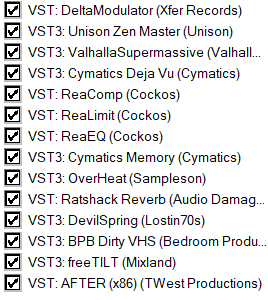
\includegraphics[width = 0.5\textwidth]{Imagenes/Bitmap/EfectosMasterEfectos.png}
    \caption{Plugins en el master con varios efectos aplicados}
    \label{fig:Efectos-master-efectos}
\end{figure}


Los efectos disponibles son los siguientes:

\begin{itemize}
    \item \textbf{Retro}: Utilizamos un plugin \textit{bitcrusher} que reduce las profundidad de bits del audio y por tanto su calidad para simular el sonido de una consola antigua. 
    \item \textbf{Bajo el agua}: Utilizamos un plugin que reduce la velocidad del audio a la mitad para ralentizar el ritmo de la canción y lograr una sensación de que está sonando dentro de agua.
    \item \textbf{Lofi}: Aplicamos un filtro de lofi a la muestra que reduce la calidad de forma creativa, filtra frecuencias y añade sonidos de polvo en una grabación.
    \item \textbf{Vintage}: Utilizamos una cadena de efectos formada por una reverberación analógica, un pedal de \textit{delay}, saturación y un filtro que simula que el sonido ha pasado a través de una cinta de grabación antigua. 
    \item \textbf{Dream}: Usamos un plugin que ralentiza un poco la velocidad de la canción y un efecto de \textit{chorus} analógico que además añade desafinación ocasional al sonido.
    \item \textbf{Espacial}: Colocamos una reverberación muy grande con el \textit{Dry} a menos infinito, por lo que no suena la señal que llega al máster si no únicamente la reverberación.
\end{itemize}